\chapter{Coordinación de Protecciones}

Este capítulo analiza la coordinación entre la protección principal del circuito 10-502 ---relé AREVA MICOM~P142 instalado en la SE~Conucos--- y las protecciones del proyecto AGPE en el nodo 3272966. El análisis se fundamenta en los ajustes oficiales entregados por ESSA, en el perfil de demanda del alimentador y en los niveles de cortocircuito calculados en el punto de conexión.

\section{Ajustes del Relé de Cabecera}

La bahía CTO~10502 dispone de un relé MICOM~P142 con funciones de sobrecorriente de fase y tierra (50, 50N, 51 y 51N). Con RTC~=~60, el pickup de la función 51 equivale a 360~A en primario, mientras que la función 50-1 queda en 2160~A; para tierra, los pickups 51N y 50N corresponden a 120~A y 1200~A, respectivamente. La Tabla~\ref{tab:ajustes_p142} consolida estos ajustes, incluyendo la lógica de recierre.

\begin{table}[H]
    \centering
    \caption{Ajustes MICOM P142 --- bahía CTO 10502 (SE Conucos)}
    \label{tab:ajustes_p142}
    \begin{tabular}{ll}
    \toprule
    \textbf{Parámetro} & \textbf{Valor} \\
    \midrule
    Fabricante / modelo / serial & AREVA / MICOM P142 / 360 \\
    Tensión / RTC / RTP & 13,8 kV / 60 / 120 \\
    Funciones & 50, 50N, 51, 51N \\
    51 (fase) & 6 A sec $\rightarrow$ \textbf{360 A} prim; TMS 0,1; IEC VI \\
    50-1 (fase) & 36 A sec $\rightarrow$ \textbf{2160 A} prim; 0 s \\
    51N (tierra) & 2 A sec $\rightarrow$ \textbf{120 A} prim; TMS 0,15; IEC VI \\
    50N (tierra) & 20 A sec $\rightarrow$ \textbf{1200 A} prim \\
    Recierre 79 & 15/30 s; reset 60 s \\
    \bottomrule
    \end{tabular}
\end{table}

La curva de tiempo inverso empleada es la IEC Very Inverse, cuya expresión es:

\begin{equation}
t = TMS \times \frac{13{,}5}{(I/I_s) - 1}
\end{equation}

Esta característica define los tiempos de operación de la función 51 ante distintas multiplicidades del pickup y será utilizada más adelante para construir la curva tiempo--corriente del esquema.

\section{Demanda del Circuito vs Pickups}

Para verificar que el relé de cabecera no opera ante condiciones normales de carga ---ni ante la exportación del AGPE--- se contrastó el perfil horario de cabecera del 19/03/2024 con los umbrales de protección. La demanda máxima del día es de 70,41~A a las 12:00, mientras que el valle nocturno desciende a 26,35~A. Frente a esos valores, el pickup de fase (360~A) ofrece un margen de 5,11 veces la demanda pico, y el de tierra (120~A) un margen de 1,70. La corriente del generador referida a media tensión es de apenas 5,25~A, muy inferior al umbral de la función 51. La Tabla~\ref{tab:dem_vs_pu} y la Figura~\ref{fig:dem_vs_pu} resumen esta comparación.

\begin{table}[H]
    \centering
    \caption{Corrientes de demanda vs umbrales de protección}
    \label{tab:dem_vs_pu}
    \begin{tabular}{lcc}
\toprule
\textbf{Magnitud} & \textbf{Valor} & \textbf{Observación} \\
\midrule
$I_{\max}$ cabecera (12:00) & 70,41 A & Demanda pico \\
$I$ @ 09:00 / 15:00 & 61,05 / 68,55 A & Horas de estudio \\
$I_{\min}$ cabecera (04:00) & 26,35 A & Valle \\
Pickup 51 & 360 A & Margen $360/70{,}41 = 5,11$ \\
Pickup 51N & 120 A & Margen $120/70{,}41 = 1,70$ \\
$I_{\mathrm{gen}}$ referida a MT & 5,25 A & $\ll$ pickup 51 \\
\bottomrule
\end{tabular}

\end{table}

\begin{figure}[H]
    \centering
    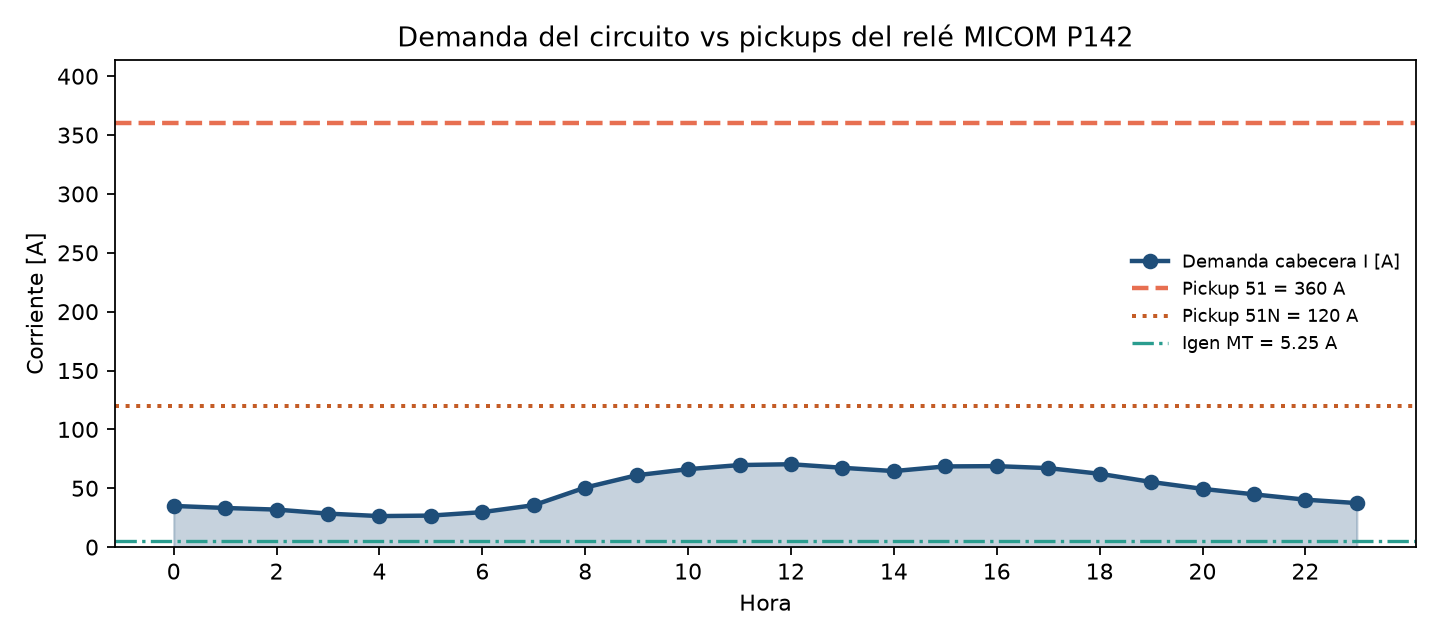
\includegraphics[width=0.95\textwidth]{figuras/fig_demanda_vs_pickup.png}
    \caption{Demanda horaria del circuito 10-502 vs pickups 51/51N e $I_{\mathrm{gen}}$ MT}
    \label{fig:dem_vs_pu}
\end{figure}

En síntesis, el pickup de fase se encuentra suficientemente alejado de la demanda máxima, y la exportación del AGPE no es capaz de operar el relé de cabecera bajo ninguna condición normal de despacho del sistema fotovoltaico.

\section{Protecciones del Proyecto AGPE}

En el lado de baja tensión del proyecto se disponen breakers de inversor (200~A por equipo) y un breaker de acometida (400~A), con disparo magnético del orden de diez veces la corriente nominal. Referidos a media tensión, estos umbrales equivalen a 3,33~A, 6,67~A y 66,7~A, respectivamente. Los inversores SOLIS aportan, además, las funciones 27, 59, 81U/O y anti-isla exigidas por la regulación. La Tabla~\ref{tab:prot_bt} consolida estos elementos.

\begin{table}[H]
    \centering
    \caption{Elementos de protección del lado BT}
    \label{tab:prot_bt}
    \begin{tabular}{lccc}
    \toprule
    \textbf{Elemento} & \textbf{Ajuste LV} & \textbf{Equiv. MT} & \textbf{Función} \\
    \midrule
    Breaker inversor (c/u) & 200 A & 3,33 A & Sobrecorriente equipo \\
    Breaker acometida & 400 A & 6,67 A & Seccionamiento POC BT \\
    Magnético acometida ($\approx 10\times$) & 4000 A & 66,7 A & Instantánea BT \\
    Inversor SOLIS & --- & --- & 27, 59, 81U/O, anti-isla \\
    \bottomrule
    \end{tabular}
\end{table}

\section{Curva Tiempo--Corriente (TCC)}

La coordinación se visualiza mediante la curva tiempo--corriente de la Figura~\ref{fig:tcc}, en la que se superponen las funciones 50/51/50N/51N del MICOM~P142 y los breakers de baja tensión referidos a media tensión. La Tabla~\ref{tab:t51} complementa el gráfico con tiempos de operación de la función 51 para distintas corrientes, desde la demanda máxima ---donde el relé no arranca--- hasta la falla trifásica en la subestación, donde opera la función instantánea.

\begin{figure}[H]
    \centering
    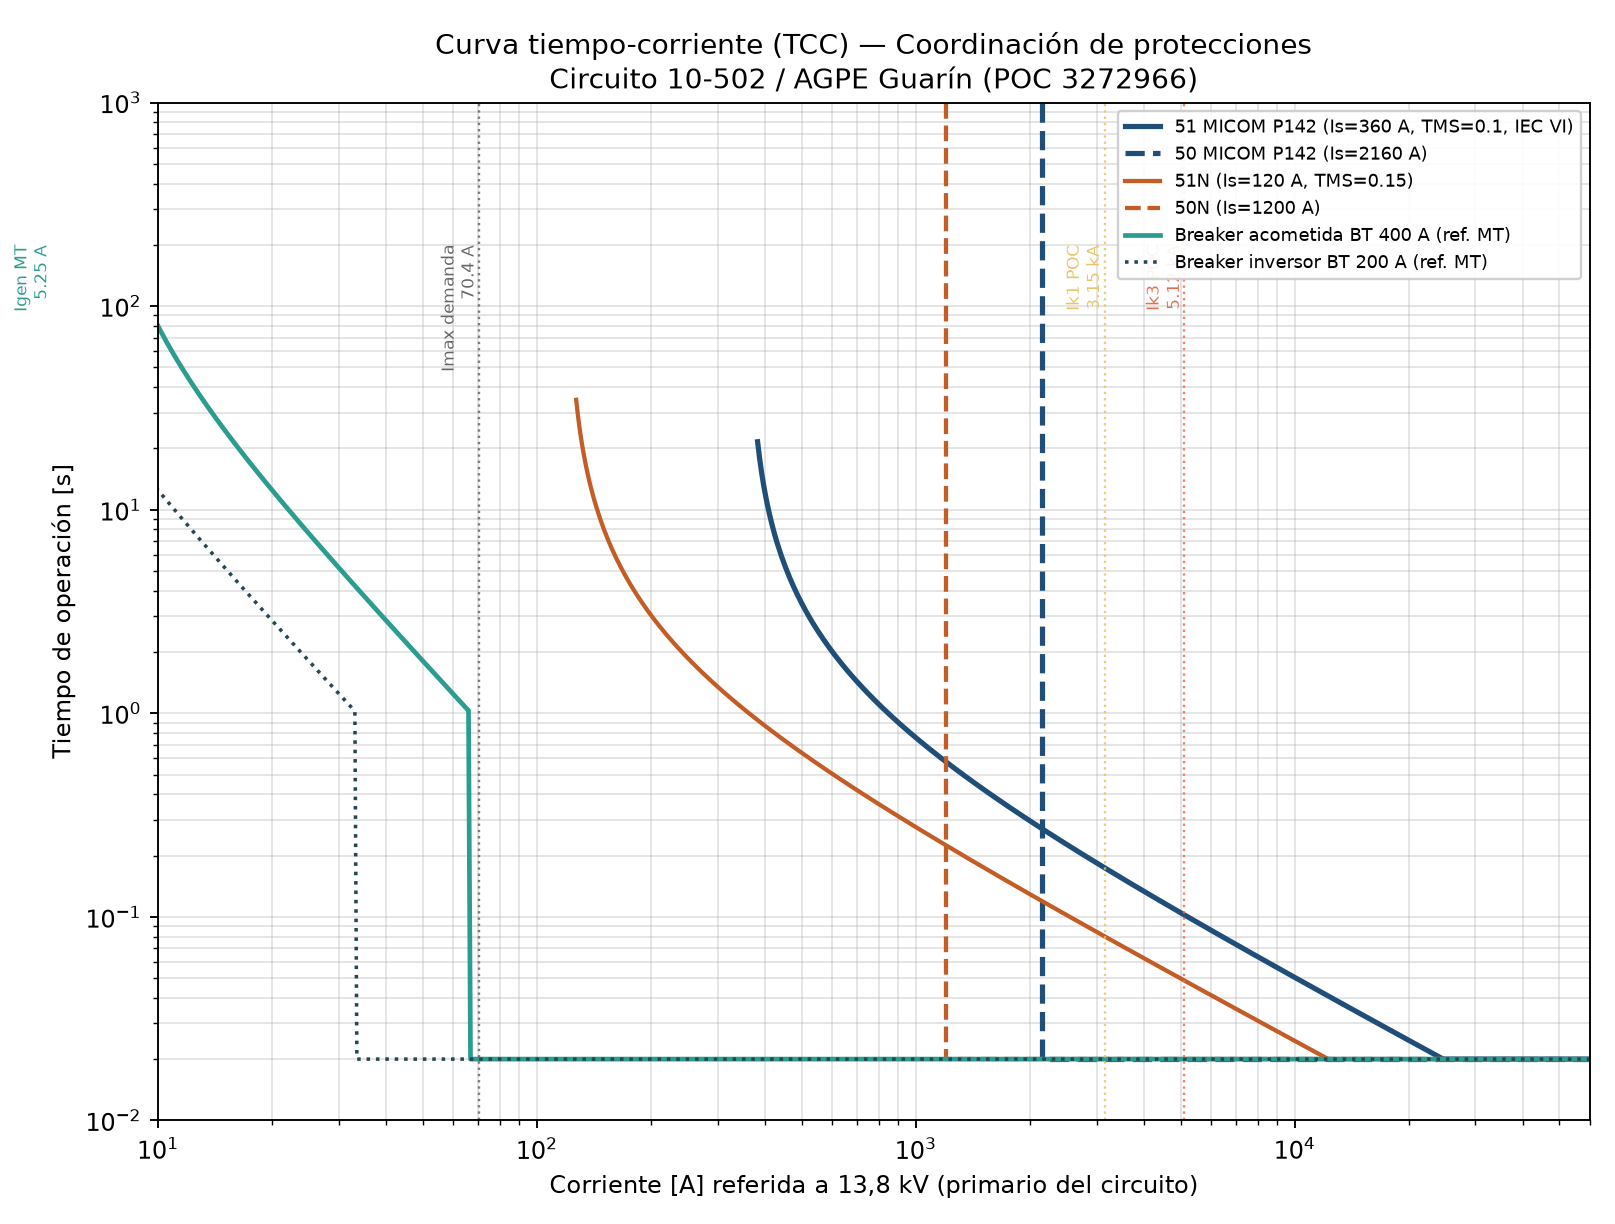
\includegraphics[width=0.98\textwidth]{figuras/fig_tcc_coordinacion.png}
    \caption{Curva TCC --- MICOM P142 (50/51/50N/51N) y breakers BT referidos a MT}
    \label{fig:tcc}
\end{figure}

\begin{table}[H]
    \centering
    \caption{Tiempos de operación de la función 51 (IEC VI, TMS $=0{,}1$, $I_s=360$~A)}
    \label{tab:t51}
    \begin{tabular}{lccc}
    \toprule
    \textbf{Condición} & \textbf{$I$ [A]} & \textbf{$t_{51}$ [s]} & \textbf{¿Opera 50?} \\
    \midrule
    $I_{\max}$ demanda & 70,4 & No arranca & No \\
    $2\times I_s$ & 720 & 1,350 & No \\
    $5\times I_s$ & 1800 & 0,338 & No \\
    $10\times I_s$ & 3600 & 0,150 & Sí \\
    $I_{k3}$ en POC & 5120 & 0,102 & Sí \\
    $I_{k3}$ en SE & 27382 & 0,020 & Sí \\
    \bottomrule
    \end{tabular}
\end{table}

\section{Selectividad BT -- MT}

Un aspecto crítico de la coordinación es garantizar que las fallas en baja tensión sean despejadas por las protecciones del proyecto, sin que el relé de cabecera arranque innecesariamente. La impedancia del transformador de 150~kVA ($Z_{cc}=4{,}9\%$) limita la corriente de una falla en BT vista desde media tensión:

\begin{equation}
Z_t = 0{,}049 \times \frac{13{,}2^2}{0{,}15} = 56{,}92~\Omega
\quad\Rightarrow\quad
I_{k,\mathrm{thru}} \approx 133{,}9~\mathrm{A}
\end{equation}

Como $I_{k,\mathrm{thru}} = 133{,}9~\mathrm{A}$ es inferior al pickup de la función 51 (360~A), el relé de cabecera \textbf{no arranca} ante fallas del lado de baja tensión. La selectividad es, por tanto, natural y total: solo operan los breakers del proyecto. La Figura~\ref{fig:margenes_prot} ilustra los márgenes de pickup y los tiempos característicos de operación asociados a este esquema.

\begin{figure}[H]
    \centering
    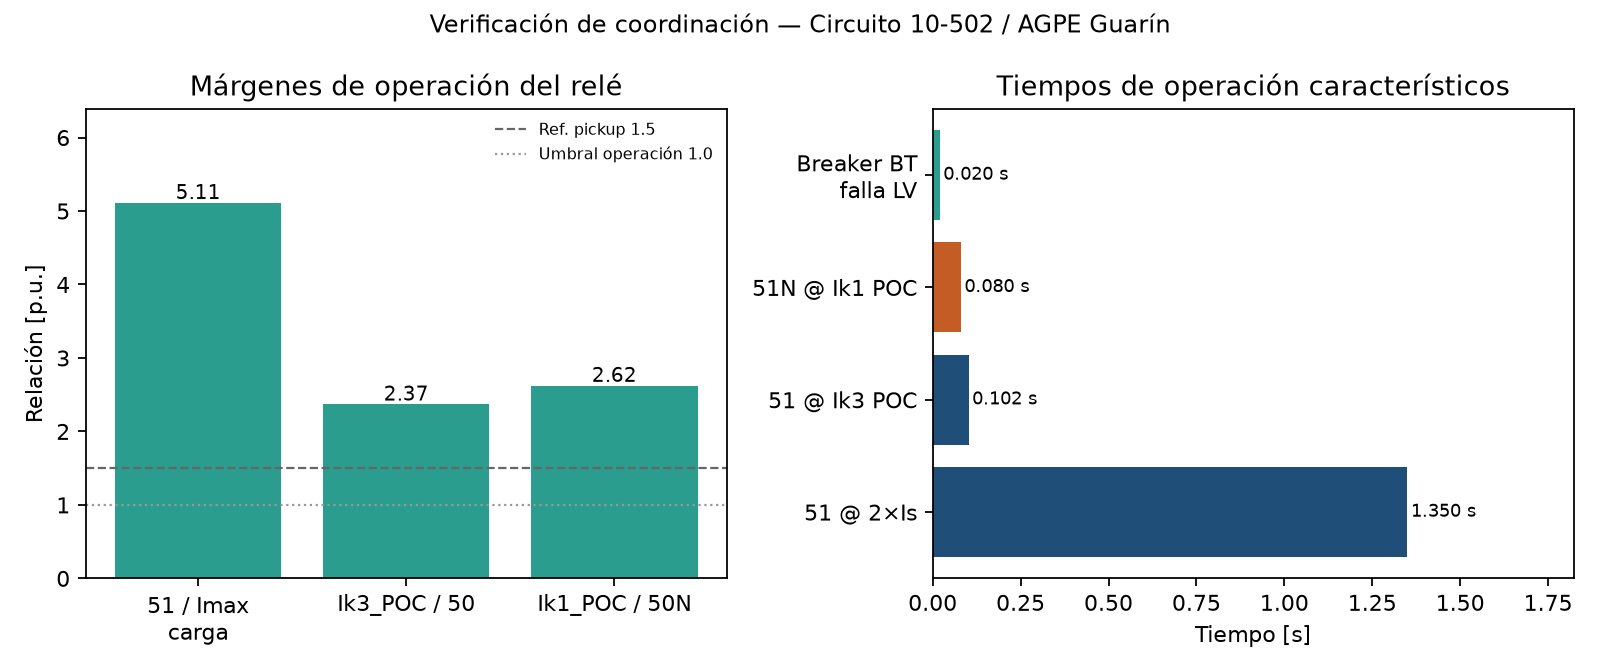
\includegraphics[width=0.95\textwidth]{figuras/fig_margenes_proteccion.png}
    \caption{Márgenes de pickup y tiempos característicos de operación}
    \label{fig:margenes_prot}
\end{figure}

\section{Respuesta ante Fallas en el POC (MT)}

Ante fallas en media tensión en el propio punto de conexión, el esquema de cabecera responde de manera adecuada. Una falla trifásica en el nodo 3272966 ($I_{k3}=5{,}12$~kA) supera el umbral de la función 50 (2160~A) y produce operación instantánea, con la función 51 actuando como respaldo en aproximadamente 0,10~s. Una falla monofásica ($I_{k1}=3{,}15$~kA) supera el umbral 50N (1200~A) y opera con un tiempo de la función 51N del orden de 0,08~s. El aporte del SSFV al cortocircuito ---7,87~A en media tensión, equivalentes al 0,15\% de $I_{k3}$ en el POC--- permanece despreciable y no altera estos tiempos ni los umbrales de disparo.

\section{Matriz de Cumplimiento}

La Tabla~\ref{tab:matriz_prot} resume los criterios de coordinación evaluados y su resultado. En todos los casos el esquema cumple: el pickup de fase supera ampliamente 1,5 veces la demanda máxima; la exportación del AGPE no dispara las funciones 51/50; el aporte de cortocircuito del SSFV es inferior al 1\%; la selectividad BT--MT está garantizada por la impedancia del transformador; y las funciones instantáneas ven las fallas de media tensión en el POC. En consecuencia, \textbf{no se requiere modificar} los ajustes del MICOM~P142.

\begin{table}[H]
    \centering
    \caption{Criterios de coordinación y resultado}
    \label{tab:matriz_prot}
    \begin{tabular}{llc}
    \toprule
    \textbf{Criterio} & \textbf{Valor} & \textbf{Resultado} \\
    \midrule
    Pickup 51 $\geq 1{,}5\times I_{\max}$ & 5,11$\times$ & Cumple \\
    Exportación AGPE no dispara 51/50 & 5,25 A $\ll$ 360 A & Cumple \\
    Aporte CC SSFV $< 1\%$ & 0,15\% & Cumple \\
    Selectividad BT vs relé cabecera & $I_{k,\mathrm{thru}}<I_{51}$ & Cumple \\
    50/50N ven fallas MT en POC & Sí & Cumple \\
    Modificar ajustes MICOM P142 & --- & \textbf{No requerido} \\
    \bottomrule
    \end{tabular}
\end{table}

\section{Conclusión de Protecciones}

La coordinación entre el AGPE Guarín y el circuito 10-502 resulta satisfactoria. No se requieren cambios en los ajustes del relé AREVA MICOM~P142. Se recomienda mantener los breakers de baja tensión en los rangos 140--200~A (inversor) y 350--500~A (acometida), y verificar en campo las funciones 27/59/81/anti-isla de los inversores SOLIS una vez el sistema entre en operación.
